\documentclass{article}

\usepackage[margin=0.75in]{geometry}
\usepackage{amsmath,amssymb}
\usepackage{graphicx,float}
\usepackage{multirow,setspace}
\usepackage{natbib,enumerate}
\usepackage{caption}
\usepackage{subcaption}
\usepackage{termcal} 
\usepackage{xcolor}
\usepackage{enumitem}
\usepackage{gensymb}
\usepackage{booktabs}
\usepackage{minted}
\usepackage{listings}

\setlength{\marginparwidth}{2cm}

\renewcommand{\thesection}{\Alph{section}}
\newcommand{\HRule}{\rule{\linewidth}{0.5mm}}
\newcommand{\tab}{\hspace{0.5cm}}
\newcommand{\modref}[1]{(\ref{#1})}

\newcommand{\bbeta}{{\mbox{\boldmath$\beta$}}}
\newcommand{\bmu}{{\mbox{\boldmath$\mu$}}}
\newcommand{\balpha}{{\mbox{\boldmath$\alpha$}}}
\newcommand{\btheta}{{\mbox{\boldmath$\theta$}}}
\newcommand{\bpi}{{\mbox{\boldmath$\pi$}}}
\newcommand{\R}{\texttt{R}}
\newcommand{\Lik}{\mathcal{L}}

\begin{document}

%%% HEADER %%%
	\begin{center}
		\HRule \\[0.1cm]
		\vspace{0.1cm}
		{ \LARGE \bfseries MATH 2625: Biostatistical Methods\\[0.5cm] Homework 1, due Thursday, January 23 } \\[0.1cm]
		\HRule \\[0.1cm]
	\end{center}
	Bailey Coughlin and Yu Fan Mei
		
	\section*{Theory}
	\begin{enumerate}
		\item Define the negative sign counting function to be
			\begin{align*}
				S^{-}(x) = \sum_{i=1}^n 1(x_i < 0).
			\end{align*}
			Show that a sign test constructed using $S^{-}(x)$ is equivalent to one we discussed in class.

			We know that when we treat $S^-(x)$ as a random variable, it takes on a binomial distribution as such:

			$$S^-(x) \sim Bin(n, p = 1/2).$$

			This is because the null hypothesis is defined As

			$$H_0 = P(x_i < 0) = 1/2.$$

			Let $s_0$ be a realization of $S^-(x)$. To calculate the p-value for the sign test, we use the following probability calculation:

			$$p = P(S^-(x) \leq s_0 | H_0) + P(S^-(x) \geq n - s_0 | H_0).$$

			Suppose, like the good mathematicians we are, we rigirously constructed this proof for the positive sign test too. Let $s_1$ be a realization of the random variable created by the positive sign counting function.

			The p-value for the positive sign test would be

			$$p = P(S^+(x) \leq s_1 | H_0) + P(S^+(x) \geq n - s_1 | H_0).$$

			Since the binomial distribution is symmetric when $p = 1/2$, this means that $p = 1 - p$. This also means that

			$$P(X = k) = P(X = n - k).$$

			This means that

			$$P(S^+(x) \leq s_1 | H_0) = P(S^-(x) \geq n - s_0 | H_0),$$

			and also that 

			$$P(S^+(x) \geq n - s_1 | H_0) = P(S^+(x) \leq s_1 | H_0).$$

			This means that the p-value generated by the positive and negative sign functions are the same.


			\newpage
		\item Consider the $p$-value constructions for both the Sign Test and Wilcoxon Signed Rank Tests:
			\begin{align*}
				p_S &= \left\{
					\begin{array}{cc}
						P(\Sigma^+ \leq S^{+}(d) | H_0) + P(\Sigma^+ \geq n - S^{+}(d) | H_0) & S^{+}(d) < \frac{n}{2}\\
						P(\Sigma^+ \geq S^{+}(d) | H_0) + P(\Sigma^+ \leq n - S^{+}(d) | H_0) & S^{+}(d) > \frac{n}{2}
					\end{array}\right.\\
				p_W &= \left\{
					\begin{array}{cc}
						P(\Omega^+ \leq W^{+}(d) | H_0) + P(\Omega^+ \geq \frac{n(n+1)}{2} - W^{+}(d) | H_0) & W^{+}(d) < \frac{n(n+1)}{4}\\
						P(\Omega^+ \geq W^{+}(d) | H_0) + P(\Omega^+ \leq \frac{n(n+1)}{2} - W^{+}(d) | H_0) & W^{+}(d) > \frac{n(n+1)}{4}
					\end{array}\right.
			\end{align*}
		
		\begin{enumerate}
			\item What value does $p_S$ or $p_W$ take on when $S^+(d) = \frac{n}{2}$ or when $W^+(d) = \frac{n(n+1)}{4}$?
			\item Can you just double the one-sided probability, i.e. the upper (or lower) tail calculation in $p_S$ or $p_W$, to attain the $p$-value? Explain why or why not.
		\end{enumerate}

		\begin{enumerate}
			\item When $S^+(d) = \frac{n}{2}$, then $p_S = 1$. When we substitute $\frac{n}{2}$ in for $S^+(d)$ (into either equation), we get
			
			$$p_S = P(\Sigma^+ \leq \frac{n}{2}|H_0) + P(\Sigma^+ \geq \frac{n}{2}|H_0 ) .$$

			Since $\Sigma^+$ is binomial, these two statements sum to 1 when $S^+(d) = \frac{n}{2}$, no matter what the size of $n$.

			We observe something similar in $p_W$, namely when $W^+(d) = \frac{n(n+1)}{4}$, $p_W = 1$. When we substitute in $W^+(d) = \frac{n(n+1)}{4}$ into the p-value constructions (either the positive or negative end), we observe

			$$p_W = P(\Omega^+ \leq \frac{n(n+1)}{4} | H_0) + P(\Omega^+ \geq \frac{n(n+1)}{2} - \frac{n(n+1)}{4} | H_0).$$

			This simplifies into

			$$p_W = P(\Omega^+ \leq \frac{n(n+1)}{4} | H_0) + P(\Omega^+ \geq \frac{n(n+1)}{4} | H_0).$$

			We can observe that this sum equals 1.

			\item Yes, we can double the one-sided probability in either test. This is because the null hypothesis $H_0$ states that the chance of having a positive or negative sign, in both the ranked and unranked sign test, is expected to be equal $(p = \frac{1}{2})$. In both of these nonparametric tests, we are calculating the probability of having this value or greater (absolutely, since it would be less if the values were negative). Since both $\Sigma^+$ and $\Omega^+$ (or their respective negatives) are symmetric, we are able to double the probability from one tail. 
		\end{enumerate}
		
	\end{enumerate}

	\section*{Case Studies}
	For each of the following, create a structured abstract no longer than 2 pages in length (including figures, tables, and references). The Background section is provided for each and should be included in your write-up. You must write the Methods, Results, and Conclusion sections.
	\begin{enumerate}
		\item In this case study, you will examine data from a crossover study examining the impact of exposure to altitude on heart rate on older and susceptible passengers. The data is in file \texttt{hrPaired.txt} where the variable \texttt{ID} denotes the subject, the variable \texttt{Control} is the average heart rate during the control day, and the variable \texttt{Flight} is the average heart rate during the flight day. Additional information of this case study is in the Background section below.
		
		\item This case study focuses on the effects of different surgical procedures on infant development as measured by the Bayley Scales. The data is in the file \texttt{heart.txt} where the variable \texttt{treatment} contains the grouping variable with the labels \texttt{DCHA} and \texttt{Low-flow} and the variable \texttt{pdi} and \texttt{mdi} contain measurements for the scales themselves. Additional information of this case study is in the Background section below.

		\newpage
		\subsection*{Background}
		
		Older and susceptible passengers and those with preexisting disease are flying with increasing frequency and in-flight cardiac emergencies are a more frequent occurrence. While commercial airplanes fly at altitudes of around 34,000 feet, Federal Aviation Administration (FAA) regulations limit cabin pressurization to an equivalent of between 7,000 and 9,000 feet, with the typical pressurization implemented by most aircraft equal to 8,000 feet. Pressurization to this equivalent level is selected to balance preventing acute altitude-related health symptoms among flyers with operational demands on the aircraft. However, comprehensive acute and longer-term health effects of cabin pressurization have not been well characterized. In particular, the impacts of short term exposure to altitude on cardiovascular health is of particular interest for study among older and vulnerable passengers. To examine possible effects, we conducted a block-randomized crossover design study of the physiological effects under simulated cabin altitudes in a hypobaric pressure chamber among such passengers. The goal of this study is to assess the changes in heart rate between simulated cabin conditions on a flight day versus control conditions. Under flight day conditions, the chamber was pressurized to the equivalent of 7,000 feet altitude. On the control days, the chamber remained at sea level.

		\subsection*{Methods}

		The trial involved 33 randomly selected participants who were older and more susceptible to in-flight cardiac emergencies. Data was analyzed at the nominal level using a paired $T$-test, with a supporting sensitivity analysis through the Wilcoxon sign-rank test. A mean baseline heart rate of 78.75 beats per minute (BPM) was observed (SD: 9.12) along with a median of 77.82 BPM and median absolute difference of 10.35 BPM. In-flight heart rate was simulated in a hypobaric pressure chamber. We observed a mean in-flight heart rate of 81.21 BPM (SD: 10.56 BPM) along with a median of 82.05 BPM. The MAD for in-flight heart rate was 14.21 BPM. We observed a mean difference between heart rates of 2.46 BPM (SD: 6.00 BPM). The median difference was 1.75 BPM, while the MAD was 5.22 BPM.

		\subsection*{Results}

		A summary of the results as stated above are provided in Table 1, including both baseline and in flight heart rates and summaries of the observed differences. Figure 1 (below) shows that these differences are fairly normal in distribution, despite the small number of participants.

		\begin{table}[h!]
			\centering
			\footnotesize
			\caption{Heart Rate Summary Statistics (in BPM)}
			\label{tab:heart_rate_summary}
			\begin{tabular}{lccc}
			\toprule
			\textbf{Measure}         & \textbf{Baseline Heart Rate} & \textbf{In-Flight Heart Rate} & \textbf{Difference} \\ 
			\midrule
			\textbf{Median}          & 77.82                        & 82.05                         & 1.750               \\ 
			\textbf{MAD}             & 10.35                        & 14.21                         & 5.22                \\ 
			\textbf{Mean}            & 78.75                        & 81.21                         & 2.462               \\ 
			\textbf{Standard Deviation} & 9.123                      & 10.560                        & 5.998               \\ 
			\bottomrule
			\end{tabular}
		\end{table}

		As shown in Table 2, we found evidence to support the claim that for people who are older and more susceptible to cardiac emergencies, their in-flight heart rate is different to their baseline heart rate $(p = 0.0246, df = 32,$ 95\% CI = $(0.335, 4.589))$. This result is consistent with the sensitivity analysis (see Table 3), which also found marginally significance in the difference between heart rates $(p = 0.0253, W = 405,$ 95\% CI = $(0.344, 4.315))$.

		\begin{table}[h!]
			\centering
			\footnotesize
			\caption{Paired T-Test Results Indicate Marginally Significant Difference in Heart Rate}
			\label{tab:t_test_results}
			\begin{tabular}{lccccc}
			\toprule
			\textbf{T-Value}  & \textbf{df} & \textbf{Mean Difference (BPM)} & \textbf{95\% Confidence Interval} & \textbf{p-value} \\
			\midrule
			2.3582      & 32          & 2.462                     & (0.335, 4.589)                    & 0.0246            \\
			\bottomrule
			\end{tabular}
		\end{table}

		\begin{table}[h!]
			\centering
			\footnotesize
			\caption{Wilcoxon Test Confirms Findings of T-Test of Significant Difference in Heart Rate}
			\label{tab:wilcoxon_results}
			\begin{tabular}{lcccc}
			\toprule
			\textbf{Test Statistic} & \textbf{Hodges-Lehmann Estimator} & \textbf{95\% Confidence Interval} & \textbf{p-value} \\
			\midrule
			W = 405                 & 2.157                           & (0.344, 4.315)                    & 0.0253            \\
			\bottomrule
			\end{tabular}
		\end{table}

			\newpage
			
			
			
			

			\begin{figure}[h!]
				\centering
				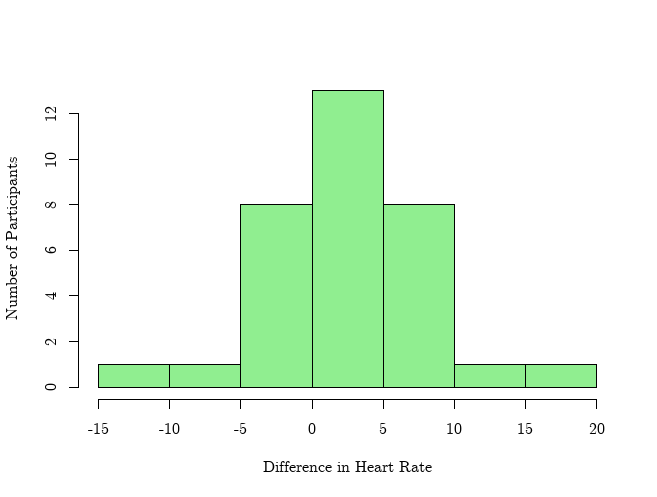
\includegraphics[width=0.6\textwidth]{HistogramCaseStudy1.png}
				\caption{Histogram of Heart Rate Differences Between Baseline and In-Flight Conditions}
				\label{fig:histogram}
			\end{figure}

			\subsection*{Discussion}
			We found a marginally significant difference between baseline and in-flight heart rates, with in-flight heart rates being slightly higher. This indicates a minor degree of cardiac instability for older and more susceptible passengers, with an association between increased heart rate. This is consistent with findings from other studies (Katoch et. al., 2024). Katoch et. al. assert that the slight tachycardia is not restricted to susceptible passengers (despite noting a severity in the change among them). Since our test only included subjects who were older and more susceptible, this was not something we could verify in our analysis. Follow-up studies should seek to examine this, potentially blocking participants into age groups or health statuses as a method of determining the differences in heart rates across different ages and susceptibilities. Further research should also seek to expand the size of the analysis overall, as the low sample size of 33 participants would have lower sensitivity and specificity than a larger sample size. Larger analyses like Toff et. al. (2006) (with an experiment size of n = 76) find robust evidence of minimal risk of cardiac emergencies at altitude, but do not offer information on heart rate variability.

			It may be also pertinent to explore the impact of 8,000 foot pressurization on acute cardiac health, given it is a more common pressurization altitude. Existing literature of 8,000 foot altitude offers conflicting conclusions. While some studies found minimal to no risk of cardiac events (Toff, et al., 2006; Bernheim, 2005), subclinical measures such as the minor heart rate increases observed in the present study have not been fully investigated. In the interim, as a hedge against extant risk of cardiac emergency, airlines may want to consider enhancing on-board cardiac care capabilities, such as stocking medical kits with HR-reducing drugs like beta blockers, which airlines are currently not required to carry (Angelo \& Dalinkus, 2023). Airlines and their passengers may also benefit from revisiting, strengthening, and clarifying their emergency policies for cardiac events.
		\newpage

		\subsection*{Background}
		
		The Bayley Scales of Infant Development yield scores on two indices---the Psychomotor Development Index (PDI) and the Mental Development Index (MDI)---that can be used to assess a child's level of functioning at approximately one year of age. As part of a study investigating the development and neurologic status of children who had undergone reparative heart congenital heart disease. Specifically, the study was on infants with D-transposition of the great arteries who underwent an arterial-switch operation. D-transposition of the great arteries is a birth defect where the child's arteries formed incorrectly and are transposed, i.e. connected to the wrong ventricles. The children in the study were randomized to one of two different treatment groups, known as ``DCHA'' and ``low-flow bypass.'' The groups differed in the specific way in which the reparative surgery was performed. Deep hypothermic circulatory arrest (DHCA) is a surgical technique that involves cooling the body to temperatures below 20\degree C (68\degree F), and stopping blood circulation and brain function for up to one hour during which time the reparative heart surgery is performed---in this case switching the ventricles the arteries are connected to. In low-flow cardiopulmonary bypass, circulation to the brain is continuously maintained, though at a reduced rate, while the reparative heart surgery is performed. While some physicians feel low-flow bypass is preferable, it has its own risks associated with brain injury. Thus, this study aims to compare PDI in the DCHA group to that in the low-flow group as well as comparing MDI between the two groups.

		\subsection*{Methods}
		Using both the PDI and MDI scales, the study tracked the psychomotor and mental development of 143 infants who underwent an arterial-switch operation. The infants were randomly assigned a treatment, with 70 receiving low-flow bypass and 73 undergoing DCHA. Analysis of the two operations were done using two-sample $T$-Tests along with a Mann-Whitney $U$ Test for sensitivity. All tests were conducted at the nominal level.

		\subsection*{Results}
		Hello 
		\begin{table}[h!]
			\centering
			\footnotesize
			\caption{Summary of Findings for Both Treatments \& Indexes}
			\label{tab:summary_statistics}
			\begin{tabular}{lcccc}
			\toprule
			\textbf{Measure}          & \textbf{PDI DCHA} & \textbf{PDI Low-flow} & \textbf{MDI DCHA} & \textbf{MDI Low-flow} \\ 
			\midrule
			\textbf{Median}           & 92.00             & 98.00                & 103.0             & 109.00              \\ 
			\textbf{MAD}              & 17.79             & 9.64                 & 16.31             & 14.08               \\ 
			\textbf{Mean}             & 91.92             & 97.77                & 103.1             & 106.40              \\ 
			\textbf{Standard Deviation} & 16.49            & 14.69                & 16.56             & 14.57               \\ 
			\bottomrule
			\end{tabular}
		\end{table}
			
			
			
		
	\end{enumerate}
		
\end{document}














